\documentclass[10pt, a4paper]{exam} 

\usepackage[brazil]{babel}
\usepackage[utf8]{inputenc}
\usepackage{listings}
\usepackage{multicol}
\usepackage{multirow}
\usepackage{caption}
\usepackage{graphicx}
\usepackage{amsmath}
\usepackage[dvipsnames]{xcolor}
\usepackage{booktabs}
\usepackage{textcomp}
%\usepackage[pdftex]{graphicx}

\lstset{ %
  language=R,                     % the language of the code
  basicstyle=\footnotesize,       % the size of the fonts that are used for the code
  numbers=left,                   % where to put the line-numbers
  numberstyle=\tiny\color{blue},  % the style that is used for the line-numbers
  stepnumber=1,                   % the step between two line-numbers. If it's 1, each line
                                  % will be numbered
  numbersep=5pt,                  % how far the line-numbers are from the code
  backgroundcolor=\color{white},  % choose the background color. You must add \usepackage{color}
  showspaces=false,               % show spaces adding particular underscores
  showstringspaces=false,         % underline spaces within strings
  showtabs=false,                 % show tabs within strings adding particular underscores
  %frame=no,                   % adds a frame around the code
  rulecolor=\color{black},        % if not set, the frame-color may be changed on line-breaks within not-black text (e.g. commens (green here))
  tabsize=2,                      % sets default tabsize to 2 spaces
  captionpos=b,                   % sets the caption-position to bottom
  breaklines=true,                % sets automatic line breaking
  breakatwhitespace=false,        % sets if automatic breaks should only happen at whitespace
  %Ttitle=\lstname,                 % show the filename of files included with \lstinputlisting;
                                  % also try caption instead of title
  keywordstyle=\color{black},      % keyword style
  commentstyle=\color{OliveGreen},   % comment style
  stringstyle=\color{YellowOrange},      % string literal style
  %escapeinside={\%*}{*)},         % if you want to add a comment within your code
  morekeywords={*,...},            % if you want to add more keywords to the set
  extendedchars=true,
  upquote=true,
  otherkeywords={\%}
} 


\extraheadheight{2cm}
\extrawidth{2cm}
\noaddpoints

\begin{document}
	\renewcommand{\solutiontitle}{\noindent\textbf{Solução:}\enspace}
	\qformat{\textbf{Questão \thequestion:}\hfill}
	\hqword{Questões} 			
	\hpgword{Páginas} 			
	%\addpoints
	\bracketedpoints
	\setlength\linefillheight{.6cm} %distância entre linhas
	
%	\pagestyle{headandfoot}
%
%	\lhead[]{}
%	\chead[]{}
%	\rhead[]{}
%	
%	\headrule
%	\footrule
%	\lfoot{}
%	\cfoot{Página \thepage\ de \numpages{}}
%	\rfoot{}
\pagestyle{headandfoot}
\lhead{\bf Universidade Estadual de Campinas - Instituto de Computação (IC/Unicamp)\\Disciplina Aprendizado de Máquina (MO444)\\ Professor: Jacques Wainer, PhD. \\Atividade 4, \today}
\chead{}
\rhead{\bf Aluno: Luiz Alberto Ferreira Gomes\\ RA:007275}

\lfoot{}
\cfoot{Página \thepage\ de \numpages{}}
\rfoot{}
	\vspace{0.1in}
	\printanswers
	
	\begin{questions}	    
	    \question
	    Use alguma metrica interna (algum Dunn, Silhouette, Calinski-Harabaz index) - apenas uma -para escolher o k entre 2 e 10. 
		\begin{solution}
			A medida interna adotada no script (ver anexo I) foi a Dunn. Ela foi extraída pela função cluster.stats para selecionar o valores de \textbf{k}. A comportamento dessa medida para os valores de k (de 2 até 10) é apresentado no gráfico abaixo.
			
			
		\begin{center}
  				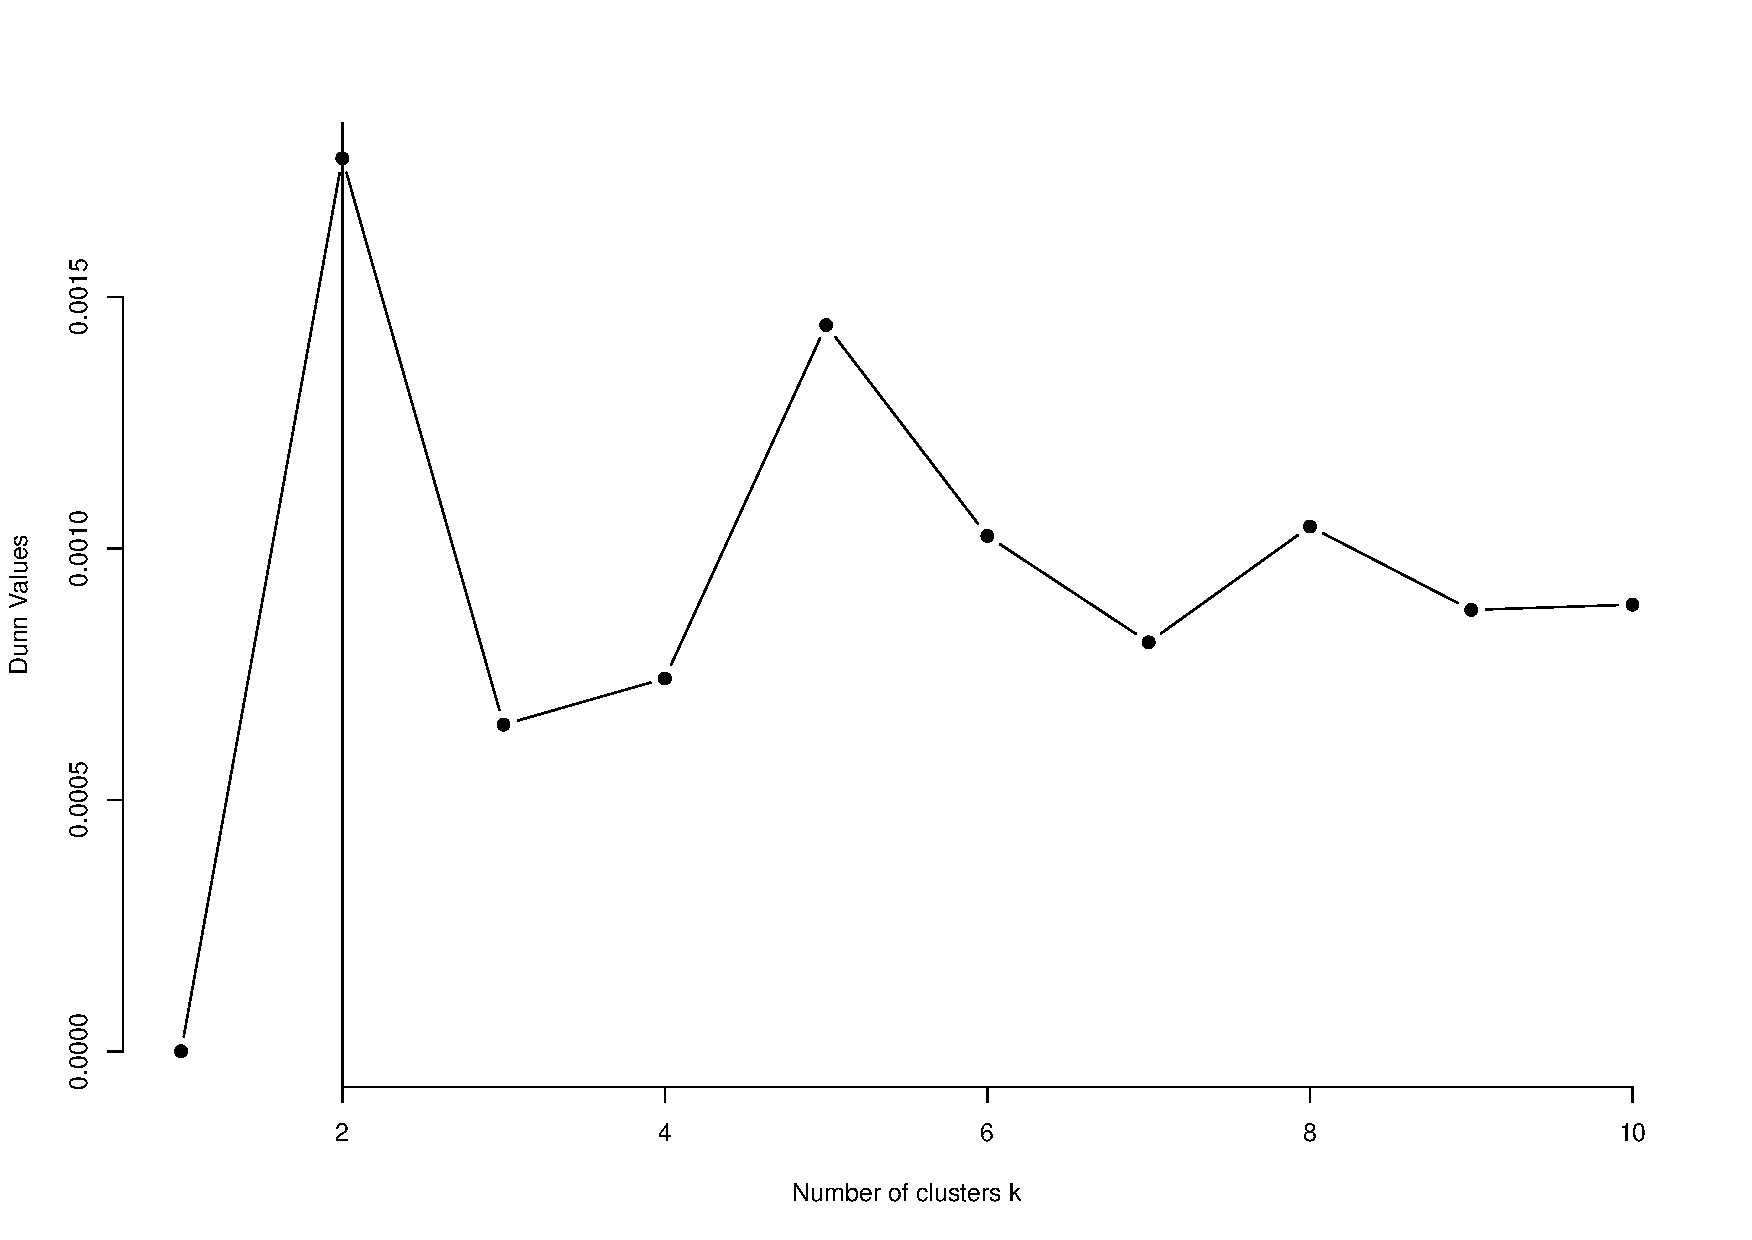
\includegraphics[scale=.5]{g1.pdf}
			\end{center}
				
		\end{solution}
		
		
	  	\pagebreak
	  	\question 
	  	Use alguma medida externa (Normalized/adjusted Rand, Mutual information, variation of information) para decidir no k.  
	    \begin{solution}
			A medida externa adotada no script (ver anexo I) foi a Ajusted Rand. Ela foi extraída pela função cluster.stats. O valor de \textbf{k} selecionado através dela foi igual a \textbf{4}, conforme o gráfico abaixo.
			
				
		\end{solution}
			\begin{center}
  				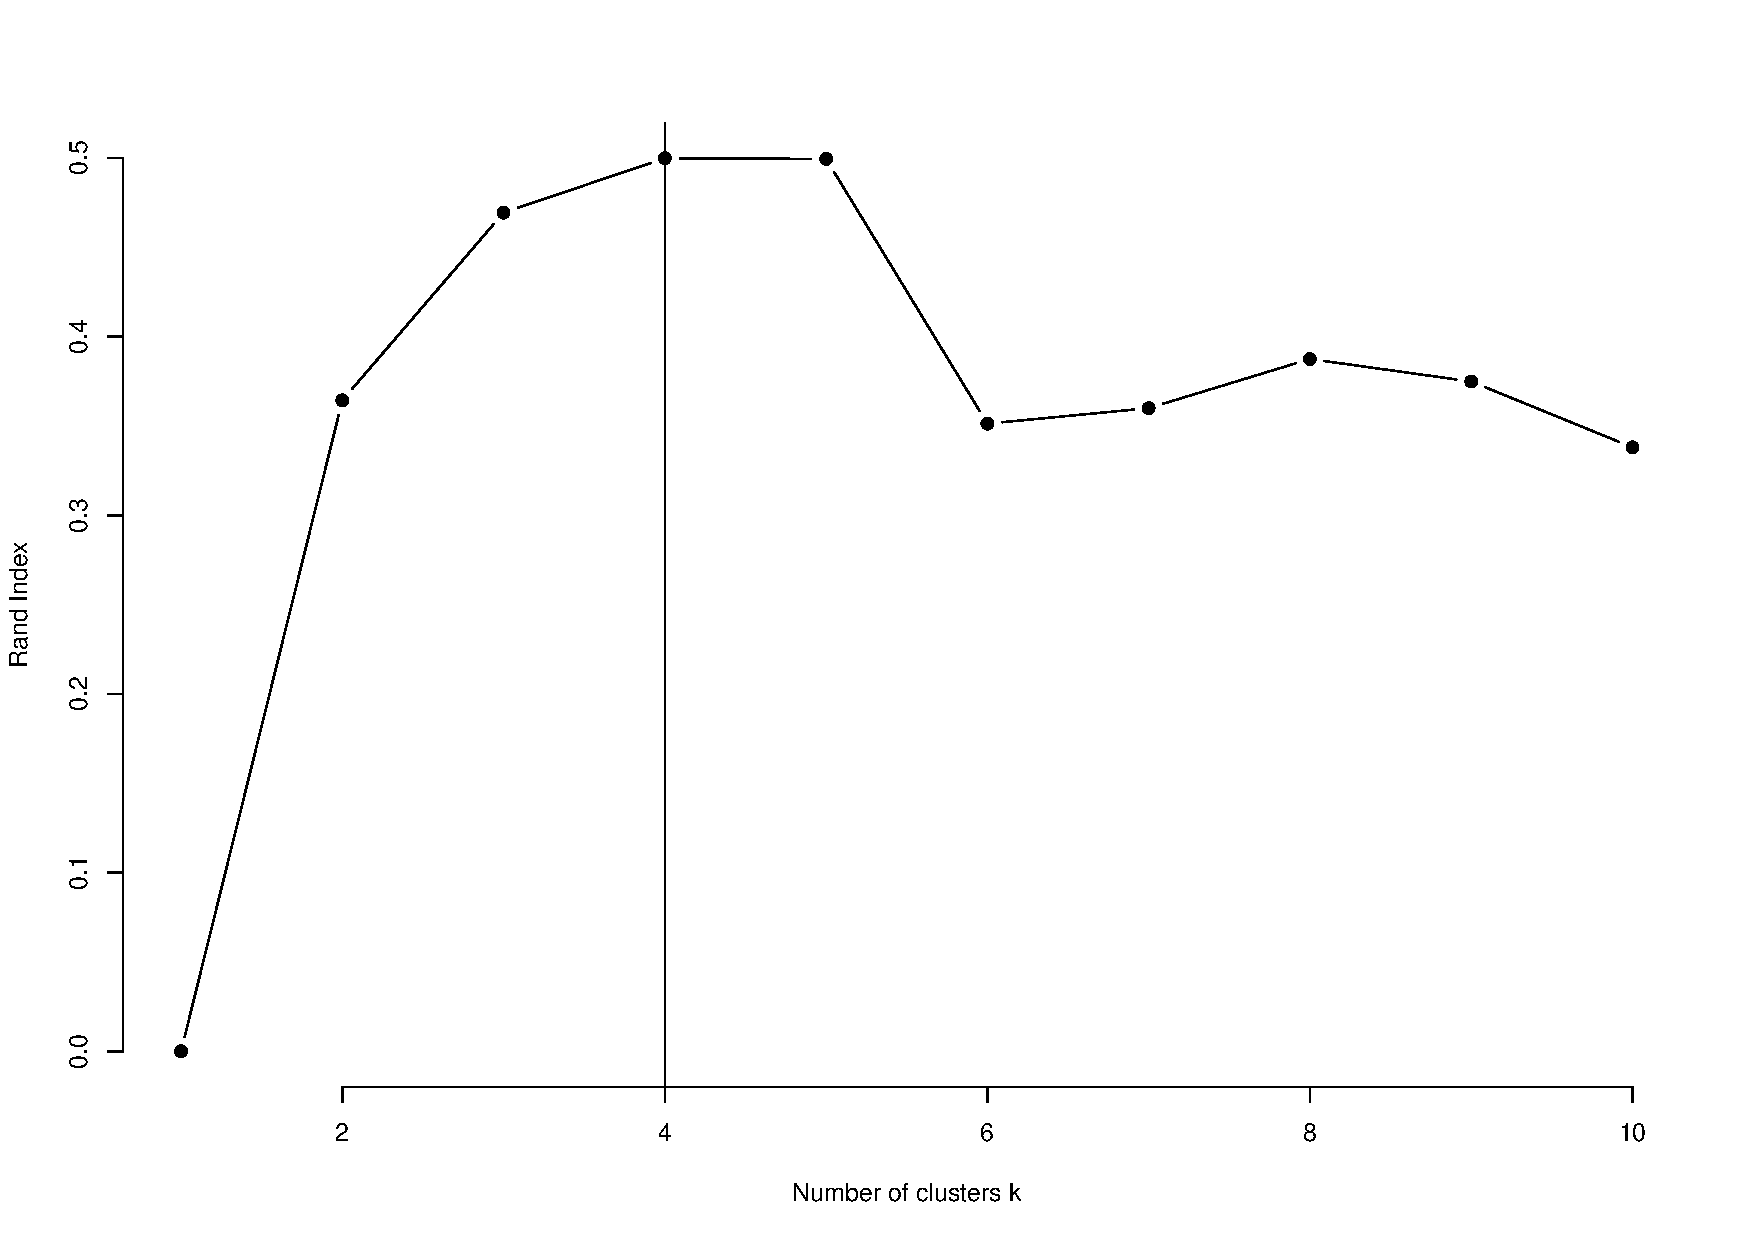
\includegraphics[scale=.5]{g2.pdf}
				\end{center}
		\paragraph{Anexo I: Script fonte em R}
		\paragraph{}
		\lstinputlisting[language=R]{solutions.3.R}

		\end{questions}
		
\end{document}
	